\documentclass[aspectratio=169]{beamer}

% Theme
\usetheme{metropolis}
\usepackage{appendixnumberbeamer}

% Packages
\usepackage{booktabs}
\usepackage{amsmath}
\usepackage{amssymb}
\usepackage{tikz}
\usetikzlibrary{arrows.meta}
\usepackage[caption=false,font=footnotesize]{subfig}
\usepackage{xcolor}

% Paths
\graphicspath{
  {../thesis/figures/}
  {../thesis/figures_paper/}
  {../paper/figures/}
}

% Colors
\definecolor{upblue}{RGB}{0, 64, 128}
\definecolor{upgold}{RGB}{180, 140, 0}
\setbeamercolor{frametitle}{bg=upblue}
\setbeamercolor{progress bar}{fg=upgold}

% Metadata
\title{Rate-Conditioned Post-Processing\\for Learned Point Cloud Compression}
\author{Spyridon Siannas}
\institute{%
  Department of Electrical \& Computer Engineering\\
  University of Patras\\[4pt]
  Supervisor: Prof.\ Konstantinos Moustakas
}
\date{Diploma Thesis Defense, 2026}

% =========================================================
\begin{document}

\maketitle

% ---------------------------------------------------------
\begin{frame}{Outline}
  \tableofcontents[hideallsubsections]
\end{frame}

% =========================================================
\section{Motivation \& Problem}

\begin{frame}{Point Clouds and Why They Need Compression}
  \begin{columns}[T]
    \column{0.55\textwidth}
    \textbf{What is a point cloud?}
    \begin{itemize}
      \item Unordered set of 3D coordinates $\{(x_i,y_i,z_i)\}$
      \item Directly acquired from LiDAR, depth cameras, photogrammetry
      \item Standard representation for volumetric video, AR/XR, autonomous vehicles
    \end{itemize}
    \vspace{6pt}
    \textbf{Why compression?}
    \begin{itemize}
      \item Single 8iVFB frame $\approx$ 800K points
      \item At 30 fps: $\sim$1.4\,GB/s raw — impractical to stream
      \item Standards: G-PCC (geometry-based), V-PCC (video projection)
      \item Learned codecs (PCGCv2, Unicorn): better rate-distortion, but\ldots
    \end{itemize}

    \column{0.42\textwidth}
    % TODO: replace with a nice point cloud photo if available
    \begin{block}{Key numbers}
      \small
      \begin{tabular}{ll}
        8iVFB resolution & $1024^3$ voxels \\
        Points per frame & up to 800K \\
        Typical low rate & 0.05 bpp \\
        Typical high rate & 0.30 bpp \\
      \end{tabular}
    \end{block}
  \end{columns}
\end{frame}

% ---------------------------------------------------------
\begin{frame}{The Oversmoothing Failure Mode}
  \begin{center}
    \includegraphics[width=0.95\textwidth]{soldier_vis.png}
  \end{center}
  \vspace{-4pt}
  \begin{columns}[T]
    \column{0.33\textwidth}
    \centering \textbf{Original} (79,529 pts)
    \column{0.33\textwidth}
    \centering \textbf{PCGCv2 r2} (76,058 pts)\\
    {\small edges blur, ridges flatten}
    \column{0.33\textwidth}
    \centering \textbf{Proposed} (76,058 pts)\\
    {\small fine structure recovered}
  \end{columns}
  \vspace{6pt}
  \textbf{Why it happens:} entropy model assigns high coding cost to rare occupancy
  patterns — exactly what high-curvature (edge/ridge) regions produce.
\end{frame}

% ---------------------------------------------------------
\begin{frame}{The Metric Gap}
  \begin{columns}[T]
    \column{0.55\textwidth}
    \textbf{D1 PSNR} averages error uniformly over all surface points.\\[6pt]
    A codec can:
    \begin{itemize}
      \item reconstruct flat surfaces near-perfectly
      \item erase all edges and ridges
      \item \ldots and still report high D1 PSNR
    \end{itemize}
    \vspace{6pt}
    \textbf{Observed gap (PCGCv2):}
    \begin{itemize}
      \item \textit{redandblack}: 2.4--4.5\,dB edge vs.\ flat gap
      \item \textit{soldier}: 1.7--2.5\,dB
      \item Gap \emph{increases} with rate — more bits, but still biased toward flat
    \end{itemize}

    \column{0.42\textwidth}
    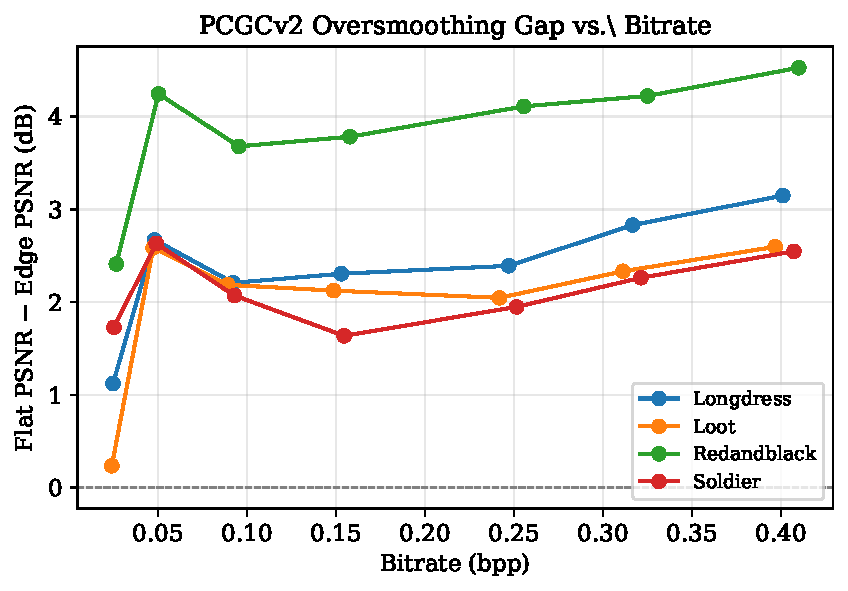
\includegraphics[width=\textwidth]{oversmoothing_gap_pcgcv2.png}
    {\small Edge vs.\ flat PSNR gap across rate points}
  \end{columns}
\end{frame}

% ---------------------------------------------------------
\begin{frame}{Research Contributions}
  \begin{enumerate}
    \item \textbf{Rate-conditioned post-processing network}\\
          FiLM-modulated sparse U-Net head. Single 2.5M-param model handles
          multiple bitrates — no retraining per rate.

    \vspace{8pt}
    \item \textbf{Curvature-stratified PSNR metric}\\
          Separately evaluates edge and flat surface regions. Exposes systematic
          degradation that aggregate D1 PSNR masks.

    \vspace{8pt}
    \item \textbf{Coordinate-only features beat curvature-augmented features}\\
          The backbone encodes local geometry from voxel positions; adding
          explicit curvature noise hurts at the boundaries where corrections
          matter most.
  \end{enumerate}

  \vspace{8pt}
  \begin{alertblock}{One-line framing}
    We \emph{diagnose} the problem, propose a \emph{metric} to measure it,
    and build a \emph{model} to fix it.
  \end{alertblock}
\end{frame}

% =========================================================
\section{Background}

\begin{frame}{PCGCv2 and Sparse Convolutions}
  \begin{columns}[T]
    \column{0.55\textwidth}
    \textbf{PCGCv2 (Wang et al., 2021)}
    \begin{itemize}
      \item Multi-scale sparse convolutional autoencoder
      \item Voxelizes geometry $\to$ occupancy grid $\to$ latent $\to$ arithmetic coding
      \item Decoder inverts: latent $\to$ reconstructed occupancy $\to$ point cloud
    \end{itemize}
    \vspace{6pt}
    \textbf{Minkowski Engine}
    \begin{itemize}
      \item Sparse tensors: only occupied voxels stored
      \item Enables 3D convolutions at $1024^3$ resolution
      \item Our post-processor uses the same engine
    \end{itemize}

    \column{0.42\textwidth}
    \begin{block}{Rate points used}
      \small
      \begin{tabular}{lll}
        \toprule
        Point & bpp & Use \\
        \midrule
        r2 & 0.05 & train + eval \\
        r4 & 0.15 & train + eval \\
        r6 & 0.30 & train + eval \\
        \bottomrule
      \end{tabular}
    \end{block}
    \vspace{4pt}
    {\small r2 = most compressed, most oversmoothed}
  \end{columns}
\end{frame}

% ---------------------------------------------------------
\begin{frame}{Feature-wise Linear Modulation (FiLM)}
  \begin{columns}[T]
    \column{0.55\textwidth}
    \textbf{Core idea:} condition a network on an auxiliary scalar by affinely
    modulating its feature maps:
    \[
      \mathbf{h}' = \boldsymbol{\gamma}(r) \odot \mathbf{h} + \boldsymbol{\beta}(r)
    \]
    \begin{itemize}
      \item $r = \log_2(\mathrm{bpp})$ — per-frame, computed from actual bitstream
      \item $\boldsymbol{\gamma}, \boldsymbol{\beta} \in \mathbb{R}^{32}$ from a small MLP
      \item Originally proposed for visual QA (Perez et al., 2018)
    \end{itemize}
    \vspace{6pt}
    \textbf{Why it fits here:}
    \begin{itemize}
      \item Single model, multiple bitrates
      \item Rate MLP is lightweight (64 params)
      \item Modulation confined to head $\to$ rate-invariant backbone
    \end{itemize}

    \column{0.42\textwidth}
    \begin{block}{Variable-rate precedent}
      \small
      Used in image/video compression for single-model variable-rate control
      (Choi et al.\ 2019; Cui et al.\ 2021; Song et al.\ 2021)
    \end{block}
  \end{columns}
\end{frame}

% =========================================================
\section{Oversmoothing Analysis}

\begin{frame}{Curvature-Stratified PSNR Metric}
  \textbf{Curvature estimation:} PCA on $k{=}30$ nearest neighbors of each
  original point:
  \[
    \kappa(p^*) = \frac{\lambda_0}{\lambda_0 + \lambda_1 + \lambda_2}
    \quad (\lambda_0 \leq \lambda_1 \leq \lambda_2)
  \]
  Range $[0,\tfrac{1}{3}]$; higher = sharper curvature.

  \vspace{8pt}
  \textbf{Stratified PSNR:} tercile split $\to$
  \begin{itemize}
    \item \textbf{Edge PSNR} (top tercile, high $\kappa$) — ridges, corners, creases
    \item \textbf{Flat PSNR} (bottom tercile, low $\kappa$) — smooth surfaces
  \end{itemize}

  \vspace{8pt}
  \textbf{Only reverse direction} (original $\to$ reconstructed): curvature labels
  anchored to original, measures \emph{missing geometry} — the primary signature
  of oversmoothing.\\
  {\small Forward direction measures hallucinated geometry — a separate failure mode.}
\end{frame}

% ---------------------------------------------------------
\begin{frame}{Oversmoothing is Spatial and Rate-Dependent}
  \begin{columns}[T]
    \column{0.50\textwidth}
    \includegraphics[width=\textwidth]{cross_sequence_summary_rev_pcgcv2.png}
    {\small Edge vs.\ flat PSNR gap per sequence and rate (PCGCv2)}

    \column{0.47\textwidth}
    \textbf{Key findings:}
    \begin{itemize}
      \item Gap is \emph{systematic}: present in all 4 sequences
      \item Gap \emph{grows with rate} — more bits still bias toward flat
      \item G-PCC shows a \emph{different} artifact profile
    \end{itemize}
    \vspace{8pt}
    \begin{alertblock}{Design implication}
      A fixed single-rate model cannot adapt.\\
      We need \textbf{rate conditioning}.
    \end{alertblock}
  \end{columns}
\end{frame}

% ---------------------------------------------------------
\begin{frame}{Displacement Signal vs.\ Rate}
  \begin{columns}[T]
    \column{0.52\textwidth}
    Ground-truth displacement magnitudes (original $-$ decoded) vary strongly
    with rate:

    \vspace{6pt}
    \begin{tabular}{lcc}
      \toprule
      Rate & Zero fraction & Mean $|\Delta|$ \\
      \midrule
      r2 & $\sim$60\% & 0.18 vox \\
      r4 & $\sim$79\% & 0.08 vox \\
      r6 & $\sim$89\% & 0.03 vox \\
      \bottomrule
    \end{tabular}

    \vspace{8pt}
    Most post-processing value is at \textbf{r2--r4}.\\
    At r6 the displacement signal is too weak to learn from with a shared backbone.

    \column{0.45\textwidth}
    \begin{alertblock}{Training implication}
      Rate weights $[1.0,\,0.3,\,0.05]$ for r2/r4/r6.\\
      Uniform weighting lets r6 dominate (easy near-zero patches).
    \end{alertblock}
    \vspace{6pt}
    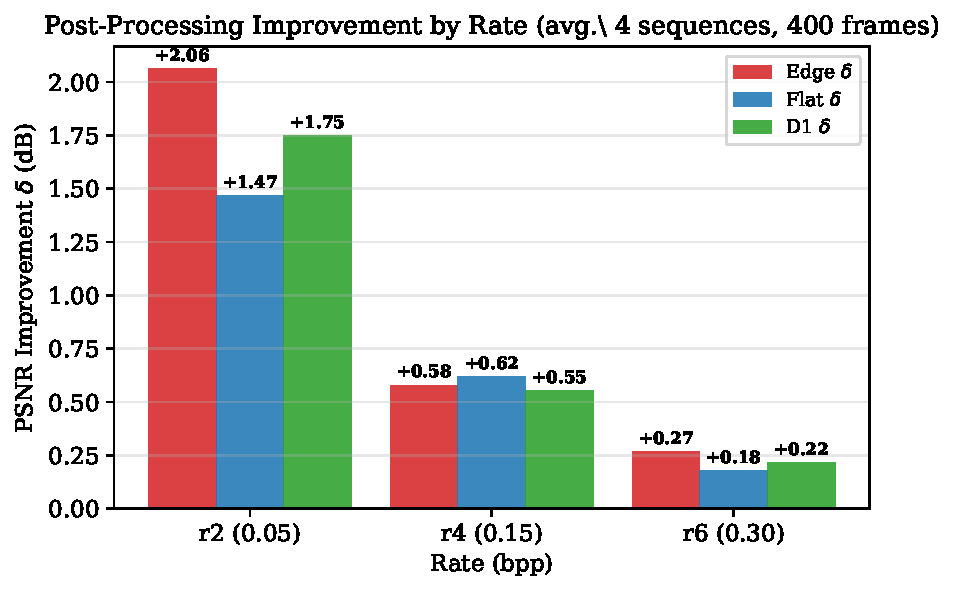
\includegraphics[width=\textwidth]{per_rate_improvement.png}
    {\small Per-rate PSNR improvement}
  \end{columns}
\end{frame}

% =========================================================
\section{Method}

\begin{frame}{Problem Formulation}
  \begin{columns}[T]
    \column{0.55\textwidth}
    \textbf{Input:} decoded point cloud $\mathbf{P} \in \mathbb{Z}^{N\times3}$,
    rate scalar $r = \log_2(\mathrm{bpp})$

    \vspace{8pt}
    \textbf{Output:} refined cloud $\hat{\mathbf{P}} = \mathbf{P} + \Delta$

    \vspace{4pt}
    $\Delta \in \mathbb{R}^{N\times3}$ are predicted displacement vectors.\\
    Point count preserved: $|\hat{\mathbf{P}}| = |\mathbf{P}|$.

    \vspace{8pt}
    \textbf{What this can and cannot fix:}
    \begin{itemize}
      \item[\checkmark] Misplaced points (displacement errors)
      \item[$\times$] Wholly missing points (occupancy errors)
      \item[$\times$] Spurious hallucinated points
    \end{itemize}

    \column{0.42\textwidth}
    \begin{block}{Why displacement?}
      \small
      At low bitrates, most decoded points have a nearby counterpart in the
      original; they are just slightly displaced. The model corrects these
      small positional errors without changing point count.
    \end{block}
  \end{columns}
\end{frame}

% ---------------------------------------------------------
\begin{frame}{Architecture}
  % Reused directly from paper/main.tex
  \resizebox{0.97\textwidth}{!}{%
  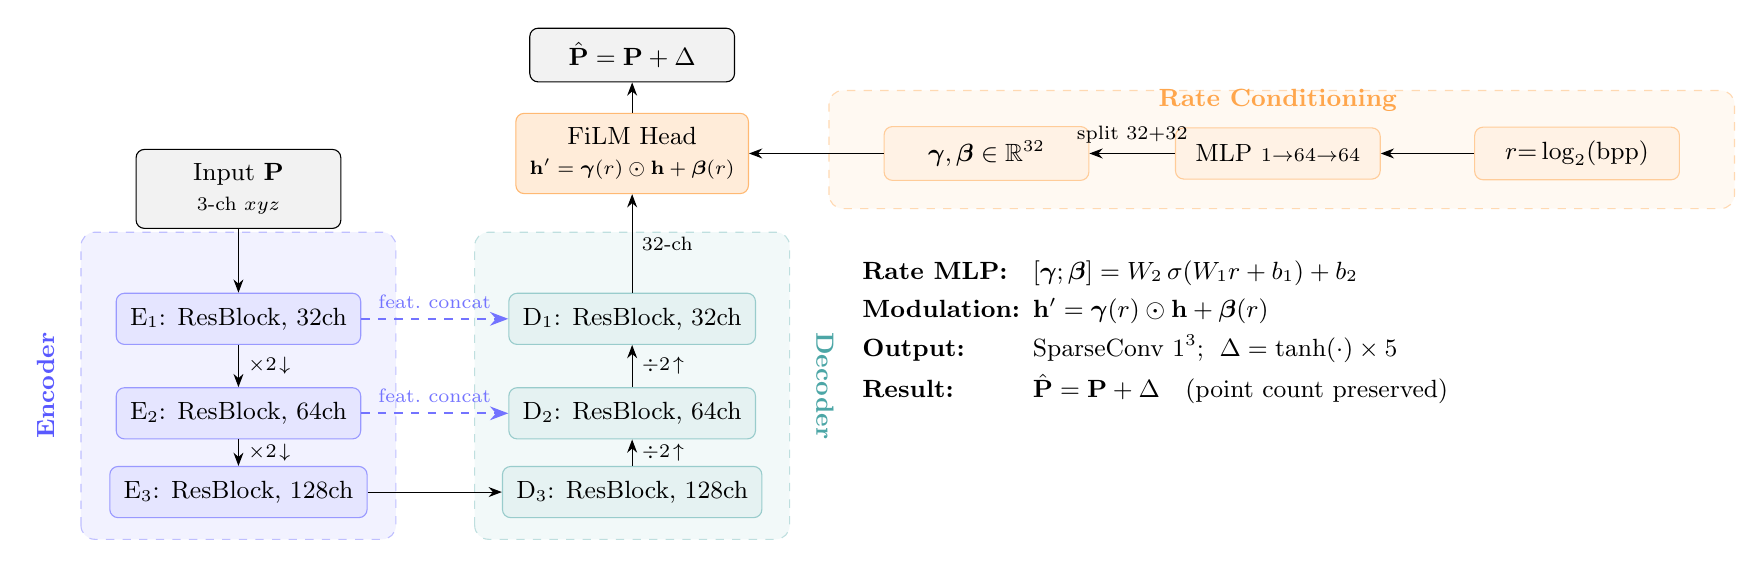
\begin{tikzpicture}[
    >=Stealth,
    every node/.style={font=\small},
    box/.style={draw, rounded corners=3pt, inner sep=5pt,
                align=center, minimum width=2.6cm, minimum height=0.65cm},
    enc/.style={box, fill=blue!10, draw=blue!40},
    dec/.style={box, fill=teal!10, draw=teal!40},
    film/.style={box, fill=orange!15, draw=orange!55},
    rate/.style={box, fill=orange!10, draw=orange!40},
    sec/.style={font=\small\bfseries},
  ]
  \draw[rounded corners=5pt, fill=blue!5, draw=blue!25, dashed]
    (-2.0,-3.6) rectangle (2.0, 0.3);
  \draw[rounded corners=5pt, fill=teal!5, draw=teal!25, dashed]
    (3.0,-3.6) rectangle (7.0, 0.3);
  \draw[rounded corners=5pt, fill=orange!5, draw=orange!30, dashed]
    (7.5, 0.6) rectangle (19.0, 2.1);
  \node[sec, blue!65,  rotate=90]  at (-2.45, -1.65) {Encoder};
  \node[sec, teal!70,  rotate=-90] at (7.45,  -1.65) {Decoder};
  \node[sec, orange!70] at (13.2, 1.97) {Rate Conditioning};
  \node[box, fill=gray!10] (P)   at (0,   0.85) {Input $\mathbf{P}$\\{\scriptsize 3-ch $xyz$}};
  \node[enc] (e1) at (0,   -0.8) {E$_1$: ResBlock, 32ch};
  \node[enc] (e2) at (0,   -2.0) {E$_2$: ResBlock, 64ch};
  \node[enc] (e3) at (0,   -3.0) {E$_3$: ResBlock, 128ch};
  \node[dec] (d3) at (5.0, -3.0) {D$_3$: ResBlock, 128ch};
  \node[dec] (d2) at (5.0, -2.0) {D$_2$: ResBlock, 64ch};
  \node[dec] (d1) at (5.0, -0.8) {D$_1$: ResBlock, 32ch};
  \node[film] (fh) at (5.0, 1.3)
    {FiLM Head\\{\scriptsize $\mathbf{h}' = \boldsymbol{\gamma}(r)\odot\mathbf{h}+\boldsymbol{\beta}(r)$}};
  \node[box, fill=gray!10] (out) at (5.0, 2.55) {$\hat{\mathbf{P}} = \mathbf{P} + \Delta$};
  \node[rate] (gb)  at (9.5,  1.3) {$\boldsymbol{\gamma},\boldsymbol{\beta}\in\mathbb{R}^{32}$};
  \node[rate] (mlp) at (13.2, 1.3) {MLP\ {\scriptsize $1{\to}64{\to}64$}};
  \node[rate] (bpp) at (17.0, 1.3) {$r{=}\log_2(\mathrm{bpp})$};
  \node[anchor=north west, font=\small] at (7.8, 0.1) {%
    \begin{tabular}{@{}l@{\enspace}l@{}}
      \textbf{Rate MLP:}    & $[\boldsymbol{\gamma};\boldsymbol{\beta}] =
                               W_2\,\sigma(W_1 r + b_1) + b_2$ \\[3pt]
      \textbf{Modulation:}  & $\mathbf{h}' = \boldsymbol{\gamma}(r)\odot\mathbf{h}+\boldsymbol{\beta}(r)$ \\[3pt]
      \textbf{Output:}      & SparseConv $1^3$;\; $\Delta = \tanh(\cdot)\times 5$ \\[3pt]
      \textbf{Result:}      & $\hat{\mathbf{P}} = \mathbf{P} + \Delta$\quad (point count preserved)
    \end{tabular}%
  };
  \draw[->] (P)  -- (e1);
  \draw[->] (e1) -- node[right]{\scriptsize $\times2\!\downarrow$} (e2);
  \draw[->] (e2) -- node[right]{\scriptsize $\times2\!\downarrow$} (e3);
  \draw[->] (e3) -- (d3);
  \draw[->] (d3) -- node[right]{\scriptsize $\div2\!\uparrow$} (d2);
  \draw[->] (d2) -- node[right]{\scriptsize $\div2\!\uparrow$} (d1);
  \draw[->] (d1) -- node[right]{\scriptsize 32-ch} (fh);
  \draw[->] (fh) -- (out);
  \draw[->, dashed, blue!55, thick] (e1.east) -- node[above]{\scriptsize feat.\ concat} (d1.west);
  \draw[->, dashed, blue!55, thick] (e2.east) -- node[above]{\scriptsize feat.\ concat} (d2.west);
  \draw[->] (bpp) -- (mlp);
  \draw[->] (mlp) -- node[above]{\scriptsize split 32+32} (gb);
  \draw[->] (gb.west) -- (fh.east);
  \end{tikzpicture}%
  }
\end{frame}

% ---------------------------------------------------------
\begin{frame}{Input Features \& Loss Function}
  \begin{columns}[T]
    \column{0.50\textwidth}
    \textbf{Input: coordinate-only (3-ch xyz)}
    \begin{itemize}
      \item Normalized $(x,y,z)$ — no explicit curvature
      \item The backbone's sparse conv receptive field already encodes local geometry
      \item Adding curvature \emph{hurts}: estimator is noisy at boundaries,
            exactly where corrections matter most \emph{(ablation result)}
    \end{itemize}

    \column{0.47\textwidth}
    \textbf{Loss: symmetric Chamfer Distance}
    \[
      \mathcal{L} = \frac{1}{|\hat{\mathbf{P}}|}\sum_{\hat{p}} \min_{p^*}\|\hat{p}-p^*\|
                  + \frac{1}{|\mathbf{P}^*|}\sum_{p^*} \min_{\hat{p}}\|p^*-\hat{p}\|
    \]
    \begin{itemize}
      \item Crops with \textbf{zero boundary padding} — avoids boundary-dominated gradients
      \item MSE discarded: too sensitive to NN assignment noise at edges
    \end{itemize}
  \end{columns}
\end{frame}

% ---------------------------------------------------------
\begin{frame}{Multi-Rate Training Strategy}
  \begin{columns}[T]
    \column{0.52\textwidth}
    \textbf{Joint training on r2 + r4 + r6}
    \begin{itemize}
      \item Batches mix rates with weights $[1.0,\,0.3,\,0.05]$
      \item Reflects declining displacement signal with rate
      \item Static choice preferred over dynamic alternatives
    \end{itemize}

    \vspace{6pt}
    \textbf{Why not dynamic weighting?}
    \begin{itemize}
      \item Kendall uncertainty: inverts ordering (weights r6 highest)
      \item Gradient-normalized: converges to near-static $[1.27, 0.91, 0.82]$
      \item Shared backbone prevents learning-speed decoupling both methods assume
    \end{itemize}

    \column{0.45\textwidth}
    \begin{block}{Training setup}
      \small
      \begin{tabular}{ll}
        Optimizer   & AdamW \\
        LR          & $5\times10^{-4}$ \\
        Weight decay & $10^{-4}$ \\
        Warmup      & 3 epochs \\
        Schedule    & Cosine (30 ep.) \\
        Batch size  & 16 \\
        GPU         & RTX 3090 \\
        Params      & 2.5M \\
        Inference   & $<$300\,ms/frame \\
      \end{tabular}
    \end{block}
  \end{columns}
\end{frame}

% =========================================================
\section{Results}

\begin{frame}{Quantitative Results}
  \begin{center}
    \begin{tabular}{lccccccccc}
      \toprule
      & \multicolumn{2}{c}{r2 (0.05\,bpp)} & \multicolumn{2}{c}{r4 (0.15\,bpp)}
      & \multicolumn{2}{c}{r6 (0.30\,bpp)} & \multicolumn{3}{c}{BD-PSNR (dB)} \\
      \cmidrule(lr){2-3}\cmidrule(lr){4-5}\cmidrule(lr){6-7}\cmidrule(lr){8-10}
      Method & Edge & Flat & Edge & Flat & Edge & Flat & D1 & Edge & Flat \\
      \midrule
      PCGCv2   & 0.00 & 0.00 & 0.00 & 0.00 & 0.00 & 0.00 & 0.00 & 0.00 & 0.00 \\
      Proposed & \textbf{+2.06} & \textbf{+1.47} & \textbf{+0.58} & \textbf{+0.62}
               & \textbf{+0.27} & \textbf{+0.18} & \textbf{+0.85} & \textbf{+0.97} & \textbf{+0.79} \\
      \bottomrule
    \end{tabular}
  \end{center}
  \vspace{6pt}
  \begin{itemize}
    \item All four 8iVFB sequences, 400 frames total
    \item Gains largest at r2: oversmoothing most severe, corrections strongest
    \item Edge gain $>$ flat gain at r2 — corrections concentrate on complex regions
    \item Monotonically decreasing with rate: rate conditioning correctly suppresses
          large displacements at higher bitrates
  \end{itemize}
\end{frame}

% ---------------------------------------------------------
\begin{frame}{Rate-Distortion Curves}
  \begin{center}
    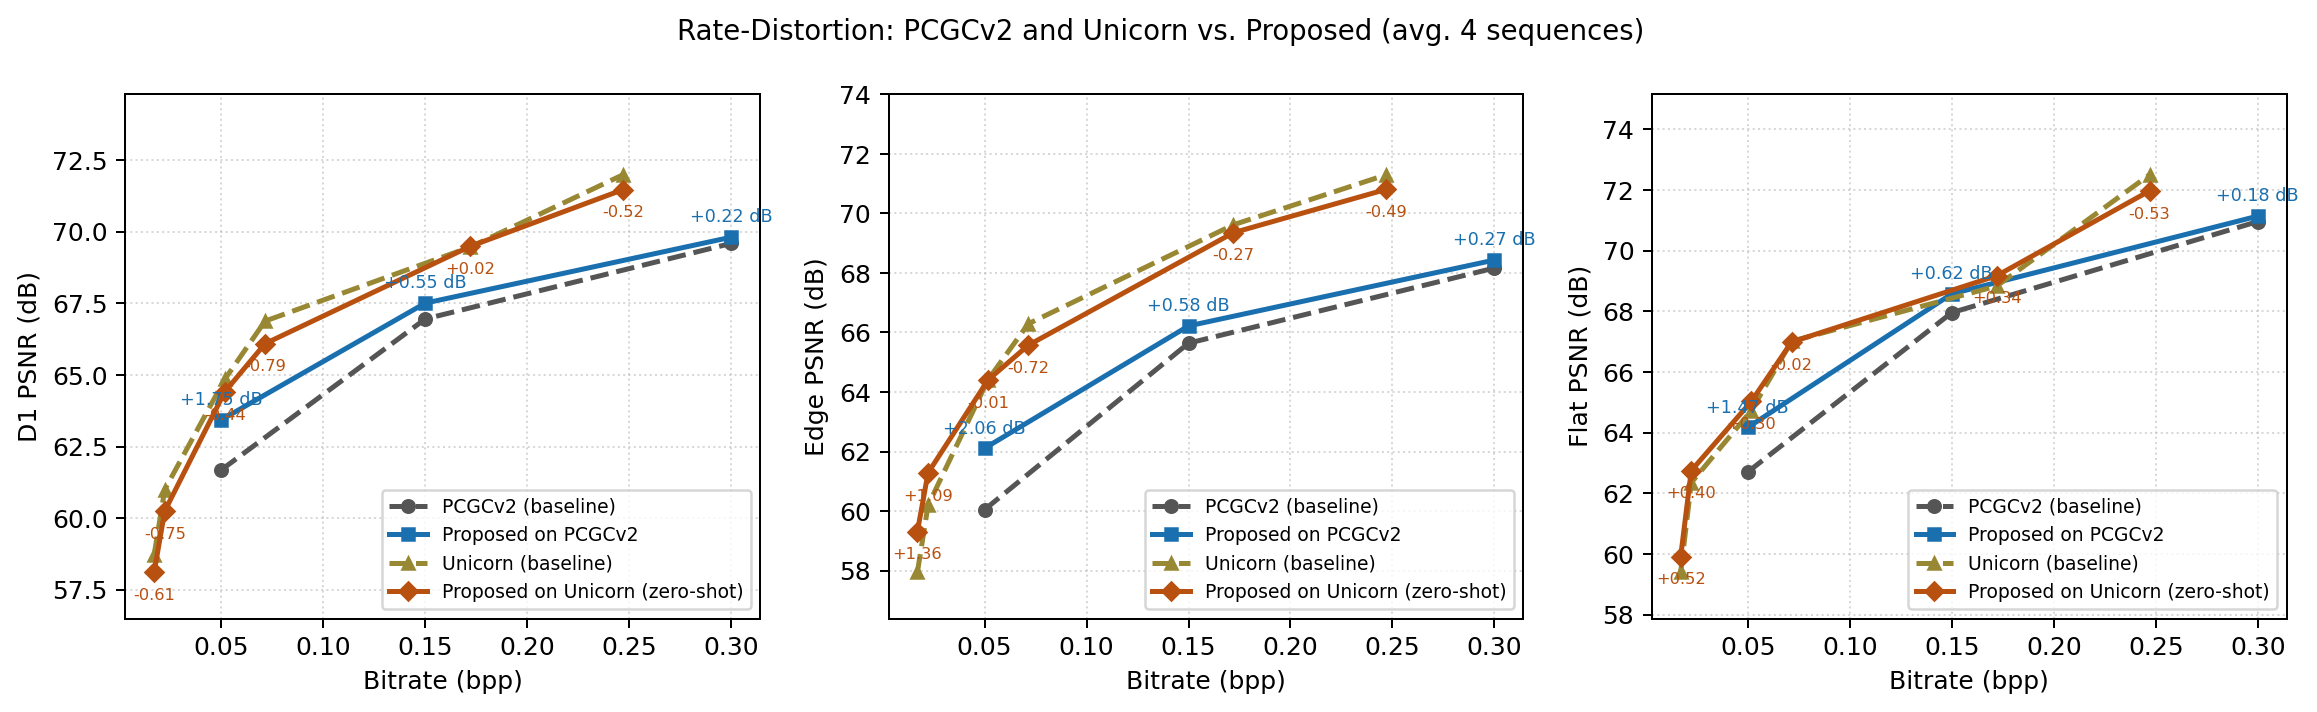
\includegraphics[width=0.93\textwidth]{rd_curve.png}
  \end{center}
  \vspace{-4pt}
  {\small Dashed = PCGCv2 baseline; solid = proposed. Orange = Unicorn zero-shot
  (R1--R6). Edge and Flat panels show the crossover around 0.05\,bpp.}
\end{frame}

% ---------------------------------------------------------
\begin{frame}{Qualitative Results}
  \begin{center}
    \includegraphics[width=0.95\textwidth]{soldier_vis.png}
  \end{center}
  \begin{columns}[T]
    \column{0.33\textwidth}
    \centering \textbf{Original}\\{\small 79,529 pts}
    \column{0.33\textwidth}
    \centering \textbf{PCGCv2 r2}\\{\small shoulder protrusions \& helmet edges merged into surrounding geometry}
    \column{0.33\textwidth}
    \centering \textbf{Proposed}\\{\small fine geometric structure substantially recovered; point count unchanged}
  \end{columns}
\end{frame}

% ---------------------------------------------------------
\begin{frame}{Ablation Study}
  \begin{center}
    \begin{tabular}{lc}
      \toprule
      Configuration & Edge $\Delta$ at r2 (dB) \\
      \midrule
      \textbf{Proposed} (3-ch xyz, FiLM head, multi-rate) & \textbf{+2.06} \\
      w/ curvature input (4-ch features)                   & +1.62 \\
      Single-rate model (r2 only)                          & +1.45 \\
      Full FiLM backbone (rate in all blocks)              & diverged \\
      \bottomrule
    \end{tabular}
  \end{center}
  \vspace{8pt}
  \begin{itemize}
    \item \textbf{Curvature input} ($-0.44$\,dB): estimator introduces noise at
          high-curvature boundaries — the regions the model most needs to correct
    \item \textbf{Single-rate} ($-0.61$\,dB): multi-rate joint training acts as a
          regularizer across rate points
    \item \textbf{Full FiLM backbone}: rate modulation in every residual block
          causes gradient interference from mixed-rate batches in shared weights;
          confining it to the head resolves this
  \end{itemize}
\end{frame}

% ---------------------------------------------------------
\begin{frame}{Cross-Codec Generalization: Unicorn}
  \textbf{Zero-shot}: model trained on PCGCv2, applied unchanged to Unicorn output.\\
  Rate conditioning uses Unicorn's actual decoded bitrate.

  \vspace{8pt}
  \begin{center}
    \begin{tabular}{llcc}
      \toprule
      Setting & Rate & Edge $\Delta$ (dB) & Flat $\Delta$ (dB) \\
      \midrule
      Unicorn R2 & 0.17\,bpp & $-0.27$ & $+0.34$ \\
      Unicorn R3 & 0.071\,bpp & $-0.72$ & $-0.02$ \\
      Unicorn R4 & 0.052\,bpp & $-0.01$ & $+0.30$ \\
      Unicorn R5 & 0.023\,bpp & $\mathbf{+1.09}$ & $\mathbf{+0.40}$ \\
      \bottomrule
    \end{tabular}
  \end{center}
  \vspace{8pt}
  \begin{itemize}
    \item Clear bitrate crossover at $\approx$0.05\,bpp
    \item Medium rates: Unicorn's distortion pattern differs from training distribution $\to$ overcorrection
    \item Extreme compression ($<$0.05\,bpp): oversmoothing artifacts become \textbf{codec-agnostic}
          $\to$ corrections transfer
  \end{itemize}
\end{frame}

% ---------------------------------------------------------
\begin{frame}{Cross-Dataset Generalization: MVUB}
  \textbf{Zero-shot}: model applied without modification to MVUB (Microsoft Voxelized
  Upper Bodies) — unseen subjects, different capture rig, $\sim$1.5M pts/frame.

  \vspace{8pt}
  \begin{center}
    \begin{tabular}{llcc}
      \toprule
      Sequence & Rate & Edge $\Delta$ (dB) & Flat $\Delta$ (dB) \\
      \midrule
      david   & r2 & $\mathbf{+0.92}$ & $\mathbf{+0.47}$ \\
      david   & r4 & $-0.46$ & $-0.06$ \\
      david   & r6 & $-0.09$ & $-0.09$ \\
      ricardo & r2 & $\mathbf{+1.03}$ & $\mathbf{+0.43}$ \\
      ricardo & r4 & $-0.50$ & $-0.14$ \\
      ricardo & r6 & $-0.12$ & $-0.12$ \\
      \bottomrule
    \end{tabular}
  \end{center}
  \vspace{8pt}
  \begin{itemize}
    \item Strong r2 result ($+$0.92--1.03\,dB): low-rate oversmoothing corrections
          transfer across human-body datasets with different capture rigs
    \item r4/r6 degradation: training weighted toward r2 + higher point density
          (1.5M vs.\ 800K) places model out of training range
  \end{itemize}
\end{frame}

% =========================================================
\section{Conclusion}

\begin{frame}{Limitations}
  \begin{columns}[T]
    \column{0.50\textwidth}
    \textbf{Fundamental constraint}
    \begin{itemize}
      \item Displacement formulation can only \emph{relocate} existing decoded points
      \item Cannot recover wholly \emph{missing} points (occupancy errors)
      \item Cannot remove \emph{hallucinated} points
      \item At very low bitrates, both types of error are present
    \end{itemize}

    \column{0.47\textwidth}
    \textbf{Training distribution}
    \begin{itemize}
      \item Rate weighting biases toward r2 $\to$ r4/r6 suffers on OOD data
      \item Small corpus: 4 sequences, $\sim$300 compressed frames
      \item Higher point density (MVUB) pushes model out of training range
    \end{itemize}
  \end{columns}
\end{frame}

% ---------------------------------------------------------
\begin{frame}{Future Work}
  \begin{enumerate}
    \item \textbf{Occupancy prediction formulation}\\
          Given a dilated neighborhood of decoded cloud as candidate voxels,
          predict binary occupancy for each candidate.\\
          Eliminates displacement targets; directly addresses occupancy errors;
          fits the integer voxel grid learned codecs operate on.

    \vspace{8pt}
    \item \textbf{Balanced multi-rate training}\\
          More training data at r4/r6; adaptive weighting strategies that
          do not conflict with shared backbone gradients.

    \vspace{8pt}
    \item \textbf{Attribute post-processing}\\
          Apply analogous rate-conditioned correction to color/normal attributes
          on top of geometry refinement.
  \end{enumerate}
\end{frame}

% ---------------------------------------------------------
\begin{frame}{Conclusion}
  \begin{block}{Summary}
    \begin{itemize}
      \item Diagnosed \textbf{spatial, rate-dependent oversmoothing} in learned
            point cloud codecs using a new curvature-stratified PSNR metric
      \item Proposed a \textbf{rate-conditioned post-processing network}:
            sparse U-Net backbone + FiLM head, coordinate-only input,
            Chamfer Distance loss
      \item A \textbf{single 2.5M-param model} operates across multiple bitrates
            without retraining
      \item \textbf{Key result}: $+2.06$\,dB edge PSNR at r2 over PCGCv2 baseline;
            $+0.85$\,dB BD-PSNR (D1)
      \item \textbf{Zero-shot transfer} to unseen codec (Unicorn) and dataset
            (MVUB) at extreme compression
    \end{itemize}
  \end{block}
  \vspace{6pt}
  \begin{alertblock}{Take-away}
    Rate-conditioning via FiLM, coordinate-only features, and Chamfer Distance
    loss is a simple, principled, and effective combination for learned-codec
    post-processing.
  \end{alertblock}
\end{frame}

% ---------------------------------------------------------
\begin{frame}[standout]
  Thank you.\\[10pt]
  \large Questions?
\end{frame}

% =========================================================
\appendix

\begin{frame}[allowframebreaks]{Backup: Curvature Metric — Full Details}
  \textbf{Curvature estimation:}
  \[
    \kappa(p^*) = \frac{\lambda_0}{\lambda_0 + \lambda_1 + \lambda_2},
    \quad \lambda_0 \leq \lambda_1 \leq \lambda_2 =
    \text{eigenvalues of } \mathrm{Cov}(\mathcal{N}_{30}(p^*))
  \]
  \textbf{Stratified PSNR:}
  \[
    \mathrm{PSNR}_s = 10\log_{10}\!\left(\frac{D_{\max}^2}{\mathrm{MSE}_s}\right),
    \quad
    \mathrm{MSE}_s = \frac{1}{|S|}\sum_{p^*\in S}\min_{\hat{p}\in\hat{\mathbf{P}}} \|p^*-\hat{p}\|_2^2
  \]
  $D_{\max} = 1023$ for 10-bit voxel grids.\\[6pt]
  \textbf{Why reverse-only?}
  \begin{itemize}
    \item Curvature labels anchored to original cloud $\to$ stratum boundaries exact
    \item Reverse measures \emph{missing geometry} (oversmoothing signature)
    \item Forward measures \emph{hallucinated geometry} — a separate failure mode
    \item Symmetric D1 mixes both; confounds post-processing evaluation
  \end{itemize}
\end{frame}

\begin{frame}{Backup: Per-Sequence Results at r2}
  \begin{center}
    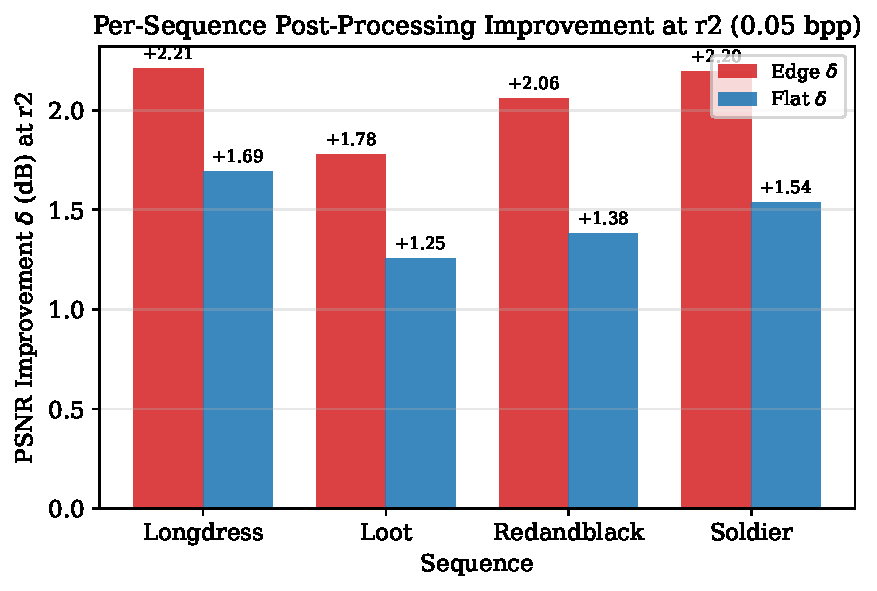
\includegraphics[width=0.85\textwidth]{per_sequence_r2.png}
  \end{center}
  {\small Edge and Flat PSNR gain at r2 per sequence. All four sequences improve.}
\end{frame}

\begin{frame}{Backup: G-PCC vs.\ PCGCv2 Oversmoothing Profile}
  \begin{center}
    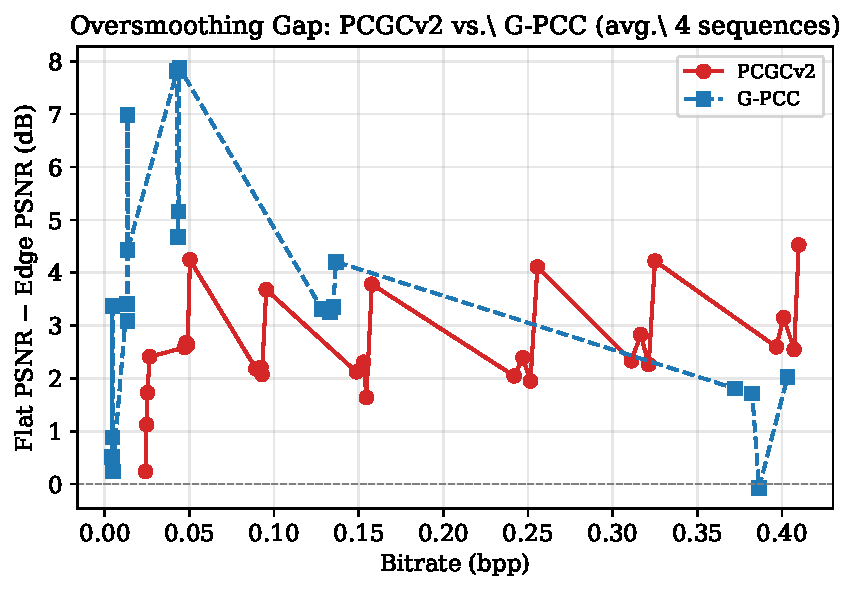
\includegraphics[width=0.85\textwidth]{gpcc_vs_pcgcv2_gap.png}
  \end{center}
  {\small G-PCC exhibits a different, lower edge--flat gap — motivation for
  targeting learned codec output specifically.}
\end{frame}

\end{document}
